\chapter{Dataset}\label{s:ds}

\section{Introduction}\label{s:ds-intro}

As I explained in the Abstract, I chose this particular dataset after having looked at many others.

An interesting one I found, for example, was DeepFashion \cite{DeepFashion2}, but it didn't feature any footwear annotations unfortunately -- which were the main focus of the task I was given. It had over 800 thousand images though!

\begin{figure}[H]
	\centering
	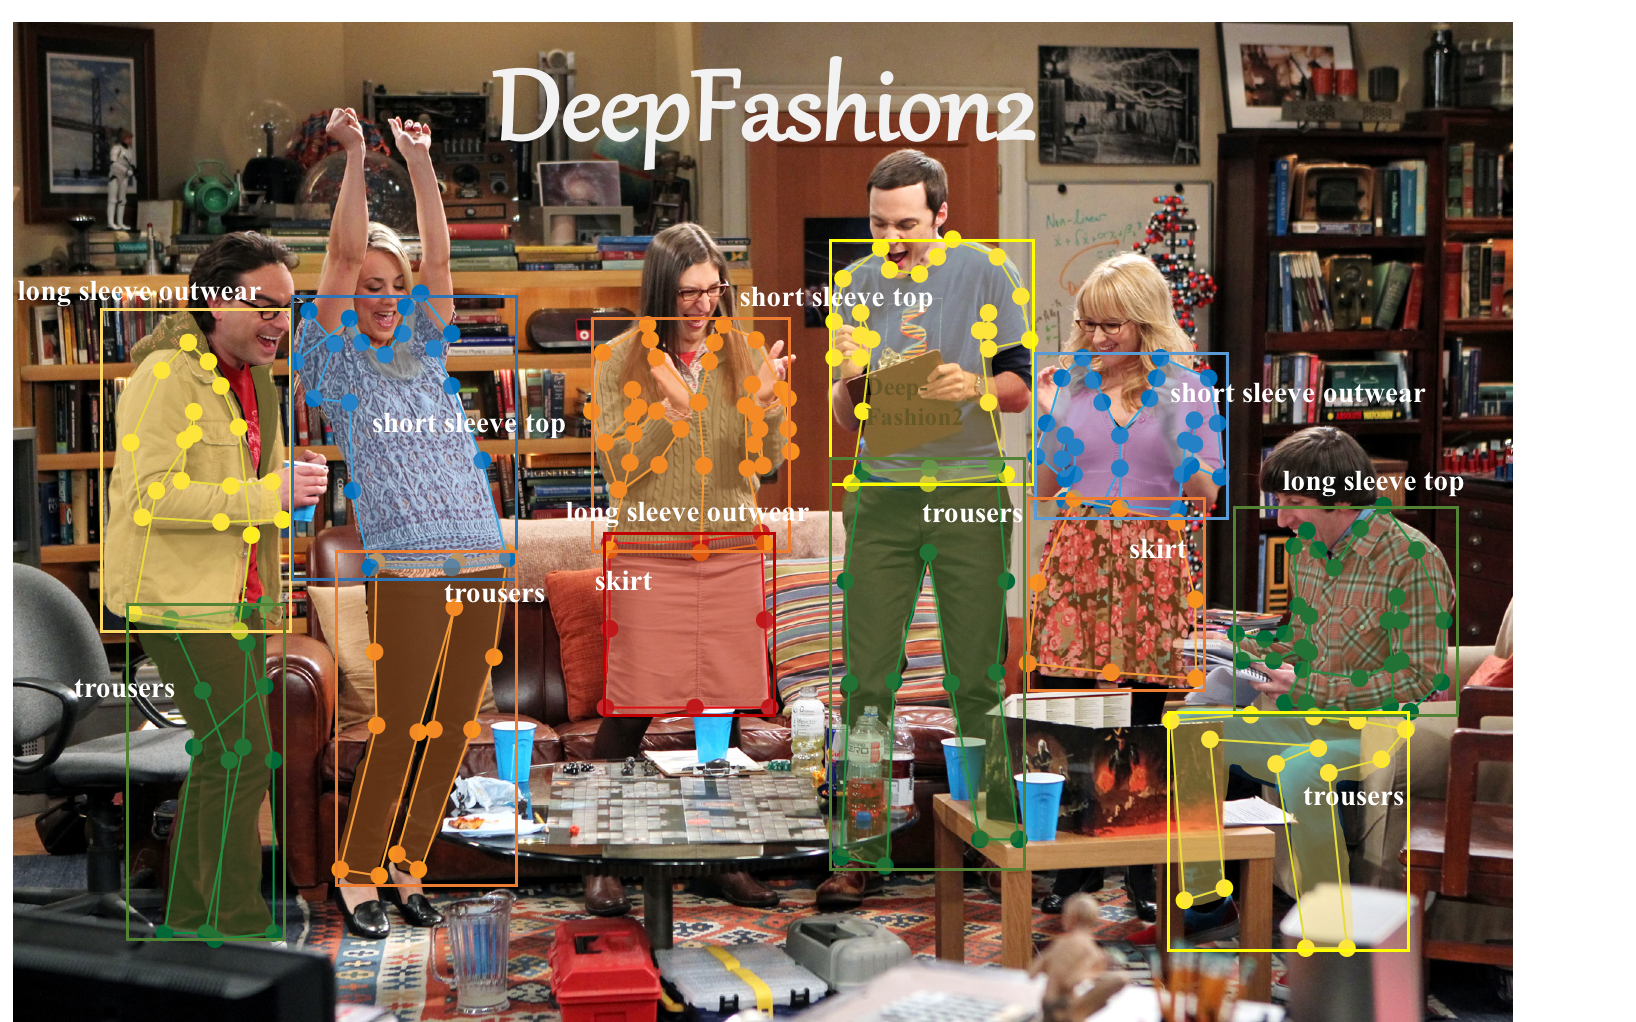
\includegraphics[width=0.75\textwidth]{images/deepfashion2_bigbang}
	\caption{DeepFashion2 feature image.}
	\label{f:deepfashion2_bigbang}
\end{figure}
As you can see below, \modanet is arguably the best for our purposes.
\begin{table}[H]
	\centering
	\caption{Comparison of ModaNet with other datasets for fashion parsing. ModaNet surpasses previous datasets in terms of annotation granularity and scale. \checkmark$^*$  indicates the annotations are not included in the original dataset. The count of categories excludes non-fashion categories, such as \emph{hair}, \emph{skin}, \emph{face}, \emph{background} and \emph{null}.}
	\label{tab:datasets}
	\begin{tabular}{@{}lcccccc@{}}
		\hline
		& DeepFashion~\cite{liu2016deepfashion} & CFPD~\cite{liu2013fashion}    & CCP~\cite{yang2014clothing}     & Fashionista~\cite{yamaguchi2012parsing} & HPW\cite{liang2015deep} & ModaNet  \\
		\hline
		\# of images      & $800,000$   & $2,682$ & $1,004$ & $685$       & $1,833$ & $55,176$ \\
		\# of categories  &     50        &     19    &      56   &       53      &  11  & 13  \\
		Pixel annotation & \texttimes      & \checkmark    &\checkmark & \checkmark      &\checkmark & \checkmark      \\
		Bounding box      & landmarks   &  \checkmark$^*$       & \checkmark$^*$         &     \checkmark$^*$         & \checkmark$^*$  & \checkmark      \\
		Polygon           & \texttimes        & \texttimes     & \texttimes     & \texttimes        &\texttimes  & \checkmark      \\ 
		\hline
	\end{tabular}
\end{table}

Then I stumbled upon this great dataset. It had much richer annotations, with \emph{almost-perfect} and very precise masks for each instance, plus it included footwear too!
\modanet has been annotated and managed by eBay researchers.
Here is their brief description of their work (on their GitHub page):
\begin{quotation}
	ModaNet is a street fashion images dataset consisting of annotations related to RGB images. ModaNet provides multiple polygon annotations for each image. This dataset is described in a technical paper with the title \emph{ModaNet: A Large-Scale Street Fashion Dataset with Polygon Annotations} \cite{zheng/2018acmmm}. Each polygon is associated with a label from 13 meta fashion categories. The annotations are based on images in the PaperDoll image set, which has only a few hundred images annotated by the superpixel-based tool. The contribution of ModaNet is to provide new and extra polygon annotations for the images.
\end{quotation}


\section{PaperDoll}\label{s:ds-paperdoll}

\section{ModaNet}\label{s:ds-modanet}

\begin{table}[H]
\centering
\small
\caption{\textbf{ModaNet labels}. Meta categories are groups of highly related raw categories}
\label{tab:modanet statistics}
\begin{tabularx}{\linewidth}{@{}lXccc@{}}
\hline
Meta & Raw & \#Train & \#Val & Avg Inst. size\\
\hline
bag  & bag & $36,699$  & $2,155$  & 4.88\% \\
belt  & belt & $13,743$ & $771$ & 0.46\% \\
boots  & boots & $7,068$ & $691$ & 2.40\%  \\
footwear  & footwear & $39,364$ & $1,617$ & 0.96\% \\
outer  & coat, jacket, suit, blazers
%, cardigan, sweater, jumpsuits, rompers, vest 
& $23,743$ & $1,358$ & 7.48\% \\
dress  & dress, t-shirt dress & $14,460$ & $804$ & 10.49\% \\
sunglasses  & sunglasses &  $8,780$ & $524$ & 0.31\% \\
pants  & pants, jeans, leggings & $23,075$  &  $1,172$ & 5.65\% \\
top  & top, blouse, t-shirt, shirt & $34,745$ & $1,862$ & 4.83\% \\ 
shorts  & shorts & $5,775$ & $429$ & 2.86\% \\ 
skirt  & skirt & $10,860$  & $555$ &  6.40\% \\ 
headwear  & headwear & $5,405$ & $491$ & 1.25\% \\ 
scarf\&tie  & scarf, tie & $3,990$ & $378$ & 2.55\%  \\ 
\hline
\end{tabularx}
\end{table}

\section{Organizing the Dataset}\label{s:ds-organizing}

\section{A Python Package to automate the process}\label{s:ds-package}